\documentclass[tikz,convert={outfile=\jobname.svg}]{standalone}
\usepackage{tikz}
\usepackage{pagecolor}
\usetikzlibrary{arrows,shapes.geometric,shapes.symbols,arrows.meta,calc,chains,scopes,shapes.misc,backgrounds}
\pgfdeclarelayer{background}
\pgfdeclarelayer{foreground}
\pgfsetlayers{background,main,foreground}
\pagecolor{white}

\tikzset{ 
   arrow/.style = {-latex,line width=0.5mm, },  
}

\begin{document}
   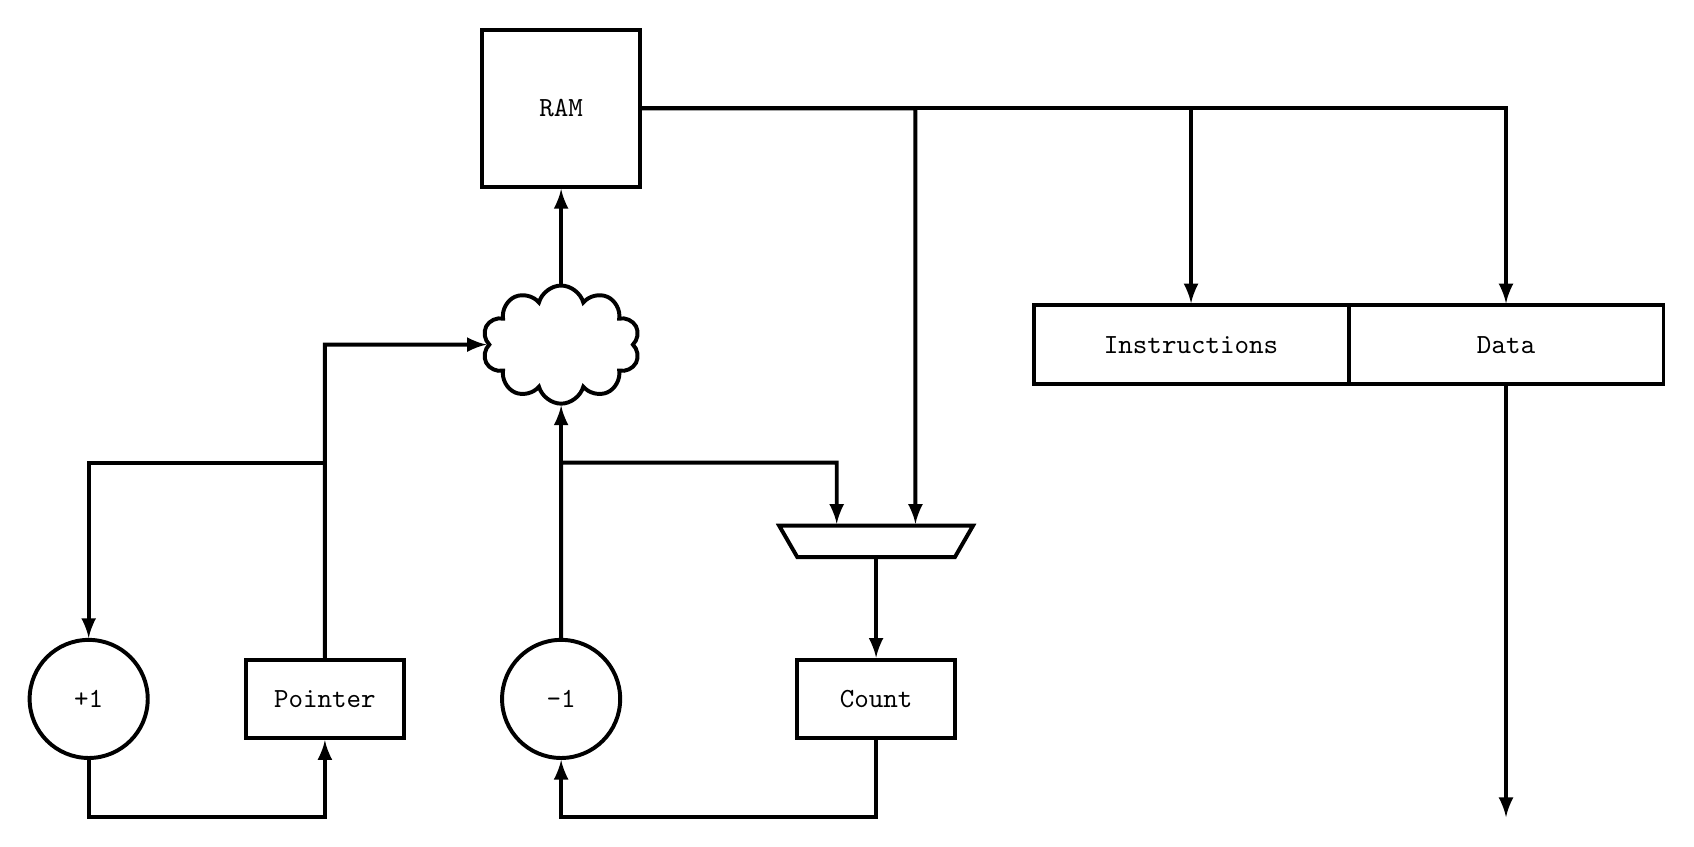
\begin{tikzpicture} 
     
      \node[
         rectangle,
         draw,
         font=\ttfamily,
         line width = 0.5mm,
         minimum height=20mm,
         minimum width=20mm,
      ] (ram) at (-70mm,40mm){RAM};

     \node[
         rectangle,
         draw,
         font=\ttfamily,
         line width = 0.5mm,
         minimum height=10mm,
         minimum width=40mm,
      ] (inst) at (10mm,10mm){Instructions};

      \node[
         rectangle,
         draw,
         font=\ttfamily,
         line width = 0.5mm,
         minimum height=10mm,
         minimum width=40mm,
      ] (data) at (50mm,10mm){Data};
 
      \node [
         trapezium,   
         draw,   
         shape border rotate = 180,  
         line width = 0.5mm,
         inner xsep=10mm,
         inner ysep=2mm,
      ] (mux) at (-30mm,-15mm) {};
        
      \node[
         rectangle,
         draw,
         font=\ttfamily,
         line width = 0.5mm,
         minimum height=10mm,
         minimum width=20mm,
      ] (cnt) at (-30mm,-35mm){Count};

      \node[
         circle,
         draw,
         font=\ttfamily,
         line width = 0.5mm,
         minimum height=15mm,
         minimum width=15mm,
      ] (subber) at (-70mm,-35mm){-1};

      \node[
         circle,
         draw,
         font=\ttfamily,
         line width = 0.5mm,
         minimum height=15mm,
         minimum width=15mm,
      ] (adder) at (-130mm,-35mm){+1};

      \node[
         rectangle,
         draw,
         font=\ttfamily,
         line width = 0.5mm,
         minimum height=10mm,
         minimum width=20mm,
      ] (ptr) at (-100mm,-35mm){Pointer};
 
       \node[
         cloud, 
         draw,
         font=\ttfamily,
         line width = 0.5mm,
         minimum height=15mm,
         minimum width=20mm,
      ] (combo) at (-70mm,10mm) {};

      \draw[arrow] (subber.north) -- (-70mm,-5mm)-- (-35mm,-5mm)  -- ([yshift=0mm,xshift=-5mm]mux.north);
      \draw[arrow] (ram.east)     -- (-25mm,40mm)  -- ([yshift=0mm,xshift=5mm]mux.north);
      \draw[arrow] (cnt.south)    -- (-30mm,-50mm) -- (-70mm,-50mm) -- (subber.south); 
      \draw[arrow] (mux.south)    -- (cnt.north);  
      \draw[arrow] (subber.north) -- (combo.south);
      \draw[arrow] (combo.north)  -- (ram.south);
      \draw[arrow] (ram.east)     -- (10mm,40mm)   -- (inst.north);
      \draw[arrow] (ram.east)     -- (50mm,40mm)   -- (data.north);
      \draw[arrow] (data.south)   -- (50mm,-50mm);
      \draw[arrow] (ptr.north)    -- (-100mm,10mm) -- (combo.west);
      \draw[arrow] (ptr.north)    -- (-100mm,-5mm) -- (-130mm,-5mm) --(adder.north);
      \draw[arrow] (adder.south)  -- (-130mm,-50mm) -- (-100mm,-50mm) --(ptr.south);



   \end{tikzpicture}
\end{document}
